\subsection{Reasoning About Efficiency}

\subsubsection{Selection Sort}

\begin{figure}[H]
  \centering
     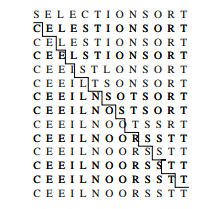
\includegraphics[scale=0.9]{./2_5.png}
  \label{fig:demo-diagram2-5}
  \caption{Animation of selection sort in action.}
\end{figure}

\begin{verbatim}
selection_sort(int s[], int n)
{
    int i, j:          /* counters */
    int min;           /* index of minimum */

    for (i=0; i<n; i++) {
        min=i;
        for(j=i+1; j<n; j++)
            if(s[j] < s[min]) min = j;
        swap(&s[i],&s[min]);
    }
}
\end{verbatim}


\subsubsection{Insertion Sort}

\begin{verbatim}
    for (i=1; i<n; i++) {
        j=i;
        while((j>0) && (s[j] < s[j-1])) {
            swap(&s[j], &s[j-1]);
            j = j-1;
        }
    }
\end{verbatim}


\subsubsection{String Pattern Matching}
\emph{Problem:} Substring Pattern Matching\\
\emph{Input:} A text string t and a pattern string p\\
\emph{Output:} Does t contain the pattern p as a substring, and if so where?\\

\begin{figure}[H]
  \centering
     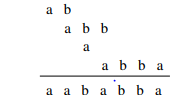
\includegraphics[scale=0.6]{./2_6.png}
  \label{fig:demo-diagram}
  \caption{Searching for the substring \emph{abba} in the text \emph{aababba}}
\end{figure}

\begin{verbatim}
int findmatch(char *p, char*t)
{
    int i, j;          /* counters */
    int m, n;          /* string lengths */

    m = strlen(p);
    n = strlen(t);

    for (i=0; i<(n-m); i=i+1) {
          j = 0;
          while((j<m) && (t[i+j] == p[j]))
              j = j + 1;
          if(j ==m) return (i);
    }

    return(-1)
}
\end{verbatim}


\subsubsection{Matrix Multiplication}

\emph{Problem:} Matrix Multiplication\\
\emph{Input:} Two matrices, A (of dimesion  $x \times y$) and B (dimension $y \times z$).\\
\emph{Output:} An $x \times z$ matrix C where C[i][j] is the dot product of the ith row of A and the jth column of B.\\
